\documentclass{article}
\usepackage{tikz}
% Ways teachers draw function graphs with TikZ, for the tests. One picture per item.
\begin{document}
\begin{enumerate}
\item Domain on the draw, x in braces.
\begin{tikzpicture}
\draw[->] (-3,0) -- (3,0) node[right] {$x$};
\draw[->] (0,-1) -- (0,5) node[above] {$y$};
\draw[domain=-2:2,smooth,variable=\x,blue] plot ({\x},{\x*\x});
\end{tikzpicture}
\item A square root that starts at a dot.
\begin{tikzpicture}
\draw (-1,0) -- (5,0); \draw (0,-1) -- (0,3);
\draw[thick,domain=0:4] plot (\x,{sqrt(\x)});
\fill (0,0) circle (2pt);
\end{tikzpicture}
\item Straight pieces.
\begin{tikzpicture}
\draw (-4,0) -- (4,0); \draw (0,-3) -- (0,3);
\draw[very thick] (-3,-1) -- (-1,2) -- (1,2) -- (3,-2);
\end{tikzpicture}
\item A jump drawn with circles.
\begin{tikzpicture}
\draw (-3,0) -- (4,0); \draw (0,-1) -- (0,4);
\draw[thick] (-2,1) -- (1,1);
\draw[thick] (1,3) -- (3,3);
\draw[fill=white] (1,1) circle (2pt);
\fill (1,3) circle (2pt);
\end{tikzpicture}
\item One formula drawn on both sides of an asymptote.
\begin{tikzpicture}
\draw (-3,0) -- (4,0); \draw (0,-4) -- (0,4);
\draw[domain=-3:0.8,samples=100] plot (\x,{1/(\x-1)});
\draw[domain=1.2:4,samples=100] plot (\x,{1/(\x-1)});
\draw[dashed] (1,-4) -- (1,4);
\end{tikzpicture}
\item Sine in radians over pi.
\begin{tikzpicture}
\draw (-3.5,0) -- (3.5,0); \draw (0,-1.5) -- (0,1.5);
\draw[domain=-pi:pi,samples=100] plot (\x,{sin(\x r)});
\end{tikzpicture}
\item Cosine with deg, over two pi.
\begin{tikzpicture}
\draw (0,0) -- (6.5,0); \draw (0,-1.5) -- (0,1.5);
\draw[domain=0:2*pi,samples=100] plot (\x,{cos(deg(\x))});
\end{tikzpicture}
\item A logarithm inside a clip.
\begin{tikzpicture}
\clip (-1,-3) rectangle (4,3);
\draw[domain=0.05:4,samples=100] plot (\x,{ln(\x)});
\end{tikzpicture}
\item Absolute value.
\begin{tikzpicture}
\draw (-3,0) -- (3,0); \draw (0,-2) -- (0,3);
\draw[domain=-3:3] plot (\x,{abs(\x)-1});
\end{tikzpicture}
\item Pieces with circle nodes for dots.
\begin{tikzpicture}
\draw (-3,0) -- (3,0); \draw (0,-1) -- (0,5);
\draw[domain=-2:0] plot (\x,{\x+2});
\draw[domain=0:2] plot (\x,{(\x)^2});
\node[circle,fill,inner sep=1.5pt] at (0,2) {};
\node[circle,draw,fill=white,inner sep=1.5pt] at (0,0) {};
\end{tikzpicture}
\item Points listed with plot coordinates.
\begin{tikzpicture}
\draw (-3,0) -- (3,0); \draw (0,-1) -- (0,4);
\draw plot coordinates {(-2,0) (0,3) (2,0)};
\end{tikzpicture}
\item A grid in help lines.
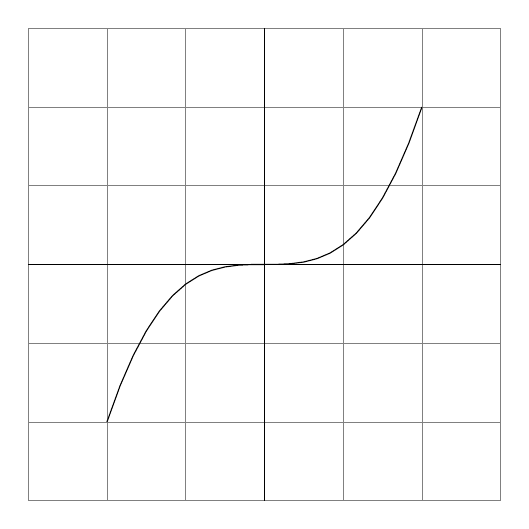
\begin{tikzpicture}
\draw[help lines] (-3,-3) grid (3,3);
\draw (-3,0) -- (3,0); \draw (0,-3) -- (0,3);
\draw[domain=-2:2] plot (\x,{\x^3/4});
\end{tikzpicture}
\item A circle drawn with two formulas.

\begin{tikzpicture}
\draw[domain=0:6.28] plot ({cos(\x r)},{sin(\x r)});
\end{tikzpicture}
\item Not a graph: a box and an arrow.
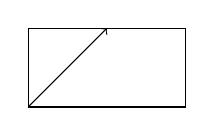
\begin{tikzpicture}
\draw (0,0) rectangle (2,1);
\draw[->] (0,0) -- (1,1);
\end{tikzpicture}
\end{enumerate}
\end{document}
